\chapter{Methodology}
This chapter discusses methodologies used throughout the project, such as the software development methodology, testing and project management used within the project.
\newline 

\section{Software Development}
The software development process was broken into the following main phases:
\begin{itemize}
    \item High Level Design – the main focus of this phase of the development was to produce an overall architecture for the system, separating the system out into its main elements and defining the clear interfaces between them. As part of this initial phase a set of screen mock-ups and associated supporting API end points were mapped out, and the initial database model design was scoped out.
    \item Low Level Design and Coding – for this phase I was able to build on the high-level design, finalising the specific design details and then code/ implement both the Frontend App and the backend server. The development of the also backend included the creation of the application database model using MySQL.
    \item Integration Testing - the main focus of this phase was to combine together the various elements and to perform a comprehensive suite of tests against the system to verify that all aspects functioned as expected.
\end{itemize}
As mentioned, the application can be broken into two sections, the frontend and the backend. As part of the coding phase the backend element of the system was developed and tested first before starting on the front end, which made it a lot easier to identify issues and fix them as they arose. 

\subsection{Backend}
To develop the backend for this project, a RESTful API was built using Node.js, Express, Sequelize and MySQL. The purpose of the backend is the manage the data for the project. This involves both the registration and login of users, and then creating, reading, updating and deleting (CRUD) data in a database. 
The development process for the backend was followed using the steps that were outlined in a tutorial found on a website. \cite{bezkoder} This tutorial allowed for a structured approach when building the backend. The tutorial covered everything from setting up the development environment to deploying the application on a server. 
\newline \newline
Before starting on the coding, the required software and tools were installed on the development machine. This included Node.js, the server-side JavaScript runtime, and the Express framework which is a fast and minimalist web framework for Node.js that is used to build web applications. MySQL, which is the database management system, was installed using the installation instructions given by the website. \cite{mySQLinstall} Once the necessary software and tools were installed, the tutorial was followed step-by-step to create the necessary files and directories for the backend application. The tutorial offered a basic structure for the application, which was then modified and expanded to meet the specific requirements for this project as shown in Figure \ref{fig:backendDirectory}
\begin{center}
    \begin{figure}[h!]
        \centering
        \label{fig:backendDirectory}
        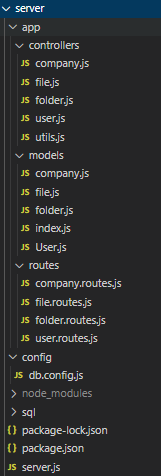
\includegraphics[height=0.40\textheight]{images/backendDirectory.png}
        \caption{Backend Directory}
    \end{figure}
\end{center}
The next step was to create a connection from the backend to the MySQL database. In order to do this, the connection information, including the database name, username and password, had to be defined in a configuration file, i.e. db.config.js. The connection to the database was then made using the Node.js MySQL driver. After the connection was made, a SQL script that specified the tables and their columns was run to create the database structure. 
\newline \newline
Following that, the API routes were then built. To be able to connect with the data in the database, a set of HTTP endpoints needed to be created. The routes were set up using the Express framework, which also dealt with HTTP requests and responses. The RESTful design of the API routes ensures that they follow a set pattern for record creation, reading, updating and deleting. To implement the CRUD operations, the Node.js MySQL driver was used to execute SQL statements that interacted with the database. The parameters given in the HTTP requests were used to generate the SQL statements on their own. This made it possible for the API to manage a variety of requests and provide the right information in response. 
\newline \newline
To ensure that the backend is reliable and well secured, various measure were taken. For example, input validation was implemented to make sure that API would only accept accurate data. Error handling was also put into place to give clients a clear error message when errors occurred. Lastly, authentication was implemented to further limit access to the API to authorised users.
Node.js was used to control the data flow across the application and speed up the request-response process. The middleware functions were used to carry out tasks like parsing incoming requests, recording requests and responses, and managing problems.
\newline \newline
Overall, the development of the backend by using the tutorial \cite{bezkoder} was a critical component of this project.  The tutorial provided a solid foundation that the developer then customized to meet the specific needs that the project entailed. The resulting RESTful API provides a secure and reliable backend for the managing of the project data.


\subsection{Frontend}
In order to develop the frontend for this project, the Expo framework was chosen due to its ease of use and efficiency in developing cross-platform applications. To set Expo up the steps outlined in the following Expo documentation was followed, \cite{buildRNscreen}. This ensured that all necessary software and tools were installed on the development machine. After the necessary software was installed, a new Expo project was created using the command-line interface that Expo provides. This is the client folder in the project. The command used to do this is \textbf{\emph{‘expo init’}} . A straightforward, simple test screen was designed by the developer to verify that the expo project was functioning.
\newline \newline
The next step was to install the React Native CLI. This involved adding React Native to the project using the command line interface and the command \textbf{\emph{‘react-native init’}}. The text editor of choice was Visual Studio Code. From the command line, this editor can be open by using the command \textbf{\emph{'code .'}} .
\newline \newline
The React Native framework was selected for its cross-platform compatibility and efficient developer process. To start on the features for the app, the developer decided to start by implementing the  Log in and Signup screens \cite{login&reg}. For these navigators were needed in the project and to use them there was a few dependencies that needed installing. Here are the sets needed for this:
\newline \newline
\begin{itemize}
    \item Change into the correct directory: 
        \begin{center}
            \begin{tcolorbox} [colback=gray!20!white,colframe=gray!50!black,width=0.5\linewidth]
                \centering\copyable{cd (Project Name) }
            \end{tcolorbox}
        \end{center}
    \item React Navigation: 
        \begin{center}
            \begin{tcolorbox} [colback=gray!20!white,colframe=gray!50!black,width=0.7\linewidth]
                \centering\copyable{‘npm install @react-navigation/native –save’}
            \end{tcolorbox}
        \end{center}
    \item Other Supporting libraries for react-navigation: 
        \begin{center}
            \begin{tcolorbox} [colback=gray!20!white,colframe=gray!50!black]
                \centering\copyable{‘npm install react-native-reanimated react-native-gesture-handler react-native-screens react-native-safe-area-context @react-native-community/masked-view –save’}
            \end{tcolorbox}
        \end{center} 
    \item Drawer Navigation: 
        \begin{center}
            \begin{tcolorbox} [colback=gray!20!white,colframe=gray!50!black,width=0.7\linewidth]
                \centering\copyable{‘npm install @react-navigation/drawer –save’}
            \end{tcolorbox}
        \end{center}
    \item Stack Navigation: 
        \begin{center}
            \begin{tcolorbox} [colback=gray!20!white,colframe=gray!50!black,width=0.7\linewidth]
                \centering\copyable{‘npm install @react-navigation/stack –save’}
            \end{tcolorbox}
        \end{center} 
    \item Install async-storage to use AsyncStorage: 
    \begin{center}
            \begin{tcolorbox} [colback=gray!20!white,colframe=gray!50!black]
                \centering\copyable{‘npm install --save @react-native-community/async-storage’}
            \end{tcolorbox}
        \end{center}
\end{itemize}
Once all dependencies where installed, React Native components were used to build the login and registration screens. The form inputs needed in these screens were managed using the \emph{‘TextInput’} component and the \emph{‘Button’} component was used for the log in and register buttons. Using the \emph{‘StyleSheet’} component the developer made the screens look appealing to use. Once this was done the next step was to create a new navigation stack by importing the \emph{‘createStackNavigation’} from \emph{@react-navigation/stack}. By using this function, it can take an object as its parameter that defines the screens and their navigation options. In this case, the two screens defined were LoginScreen and RegisterScreen. 
\newline \newline
Now the options for each screen could be defined. This covers choices such as the screen title, header design and navigational style. The screens chosen for this were the HomeScreen and the SettingsScreen. By designing basic screens the developer was then able to test if the navigation system was properly working.







\section{Project Management}
 
This section will describe the various development tools that were used throughout the period of the project's development.

\subsection{Microsoft Teams}

The Microsoft Teams application was frequently used for virtual meetings with the supervisor. In these meetings the project process from the previous week, the plan for the following week and feedback from the supervisor was discussed. Meetings with the supervisor were initially all in person but with changing time schedules they were brought online to facilitate both parties. Microsoft Teams was very beneficial for meetings as it was easy to share screens and other documents with the supervisor. There was not much difference between in person ad online meetings when using Microsoft Teams. This application allowed for a weekly scheduled meeting that was added to both developer and supervisors’ calendars. It also sent reminders 30 minutes before the meeting to both parties. However, having good internet access was a necessary requirement to be able to use the application. 

\subsection{Google Slides}

To plan the design of the app, Google slides was used to draw up wireframes. This let the user create diagrams, schemas and map out the layout for the application. Google Slides is a collaborative tool, so it was easy to share these slides with the supervisor to be able to get feedback. These diagrams are later seen in Figure \ref{image:wireframe}

\subsection{Jira}
Jira was used to implement a project management methodology. This was based on 2-week sprints. This software provided the ability to add issues to sprints at any time of the development. This meant that the planning was flexible and was able to have adjustments made when needed. Also, any tasks that were incomplete in the previous sprint was automatically carried over to the following sprint. This ensured that the project was always moving forward, and progress was not lost as the task could be complete in the next sprint. By using Jira software it meant there was a structured approach to the management of the project. It allowed for the developer to have a clear visualisation of what had to be done and allowed for easy tracking of the progress that had been made already. By being able to edit sprints and carry over unfinished tasks it made it simple to manage the project and ensured that all tasks were complete within the planned timeframe, as some weeks the developer could get more work done than others. 
\newline \newline
Additionally, with the use of epics, the user was able to break larger tasks into smaller tasks. For example when creating the Authentication part of the project, the developer could break it down into log in, log out and register. This created a high level of organisation and made it less daunting for the developer when they went to implement a large task.



